\begin{figure}[h]
    \centering
    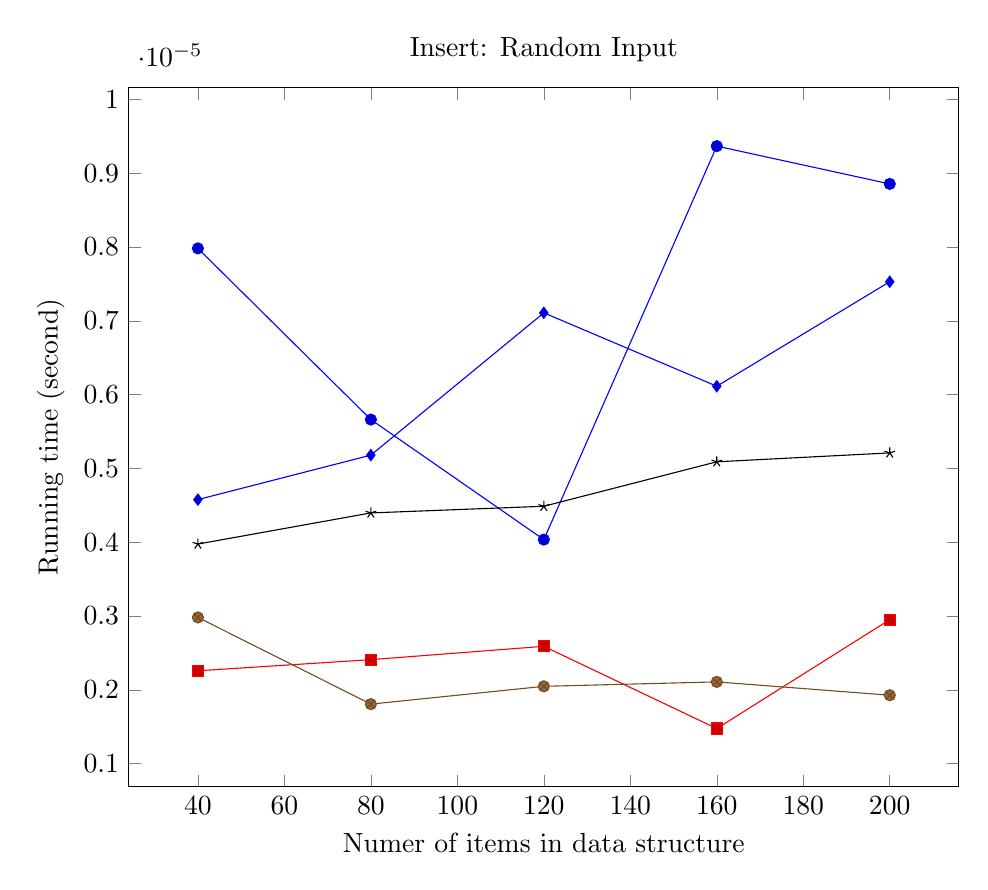
\begin{tikzpicture}
        \begin{axis}[
            xlabel={Numer of items in data structure},
            ylabel={Running time (second)},
            title={Insert: Random Input},
            width=\textwidth
        ]
		\addplot coordinates {
			(40, 7.981146423929886e-06)
			(80, 5.662096330993905e-06)
			(120, 4.035749512354414e-06)
			(160, 9.36655297287814e-06)
			(200, 8.854554900494805e-06)
		};
		\addplot coordinates {
			(40, 2.2588150255131724e-06)
			(80, 2.4094026940701953e-06)
			(120, 2.5901078959833514e-06)
			(160, 1.4757591500824673e-06)
			(200, 2.9515183001649346e-06)
		};
		\addplot coordinates {
			(40, 2.981635833521068e-06)
			(80, 1.8070520205526463e-06)
			(120, 2.0479922898886117e-06)
			(160, 2.1082273573114206e-06)
			(200, 1.9275221553982645e-06)
		};
		\addplot coordinates {
			(40, 3.975514444931605e-06)
			(80, 4.397159916535997e-06)
			(120, 4.48751251731494e-06)
			(160, 5.089863190832488e-06)
			(200, 5.210333325678107e-06)
		};
		\addplot coordinates {
			(40, 4.577865118804425e-06)
			(80, 5.180215791966703e-06)
			(120, 7.107737947364967e-06)
			(160, 6.113859336309701e-06)
			(200, 7.529383418614089e-06)
		};
        \legend{}
        \end{axis}
    \end{tikzpicture}
    \caption{Average of 0 operations, benchmarked every 0, starting at 0.}
\end{figure}